\documentclass[12pt, a4paper]{article}
\usepackage{graphicx}
\graphicspath{{assets/}}

\title{My first LaTex document}
\author{Ghribi Ouassim Abdelmalek\thanks{Hello there}}
\date{April 2024}
\begin{document}
\maketitle
First document. This is a simple example, with no
extra parameters or packages included.
% This is a comment and should not appear

Some of the \textbf{greatest}
discoveries in \underline{science}
were made by \textbf{\textit{accident}}.

Some of the greatest \emph{discoveries} in science
were made by accident.

\textit{Some of the greatest \emph{discoveries}
    in science were made by accident.}

\textbf{Some of the greatest \emph{discoveries}
    in science were made by accident.}


\begin{figure}[h]
    \centering
    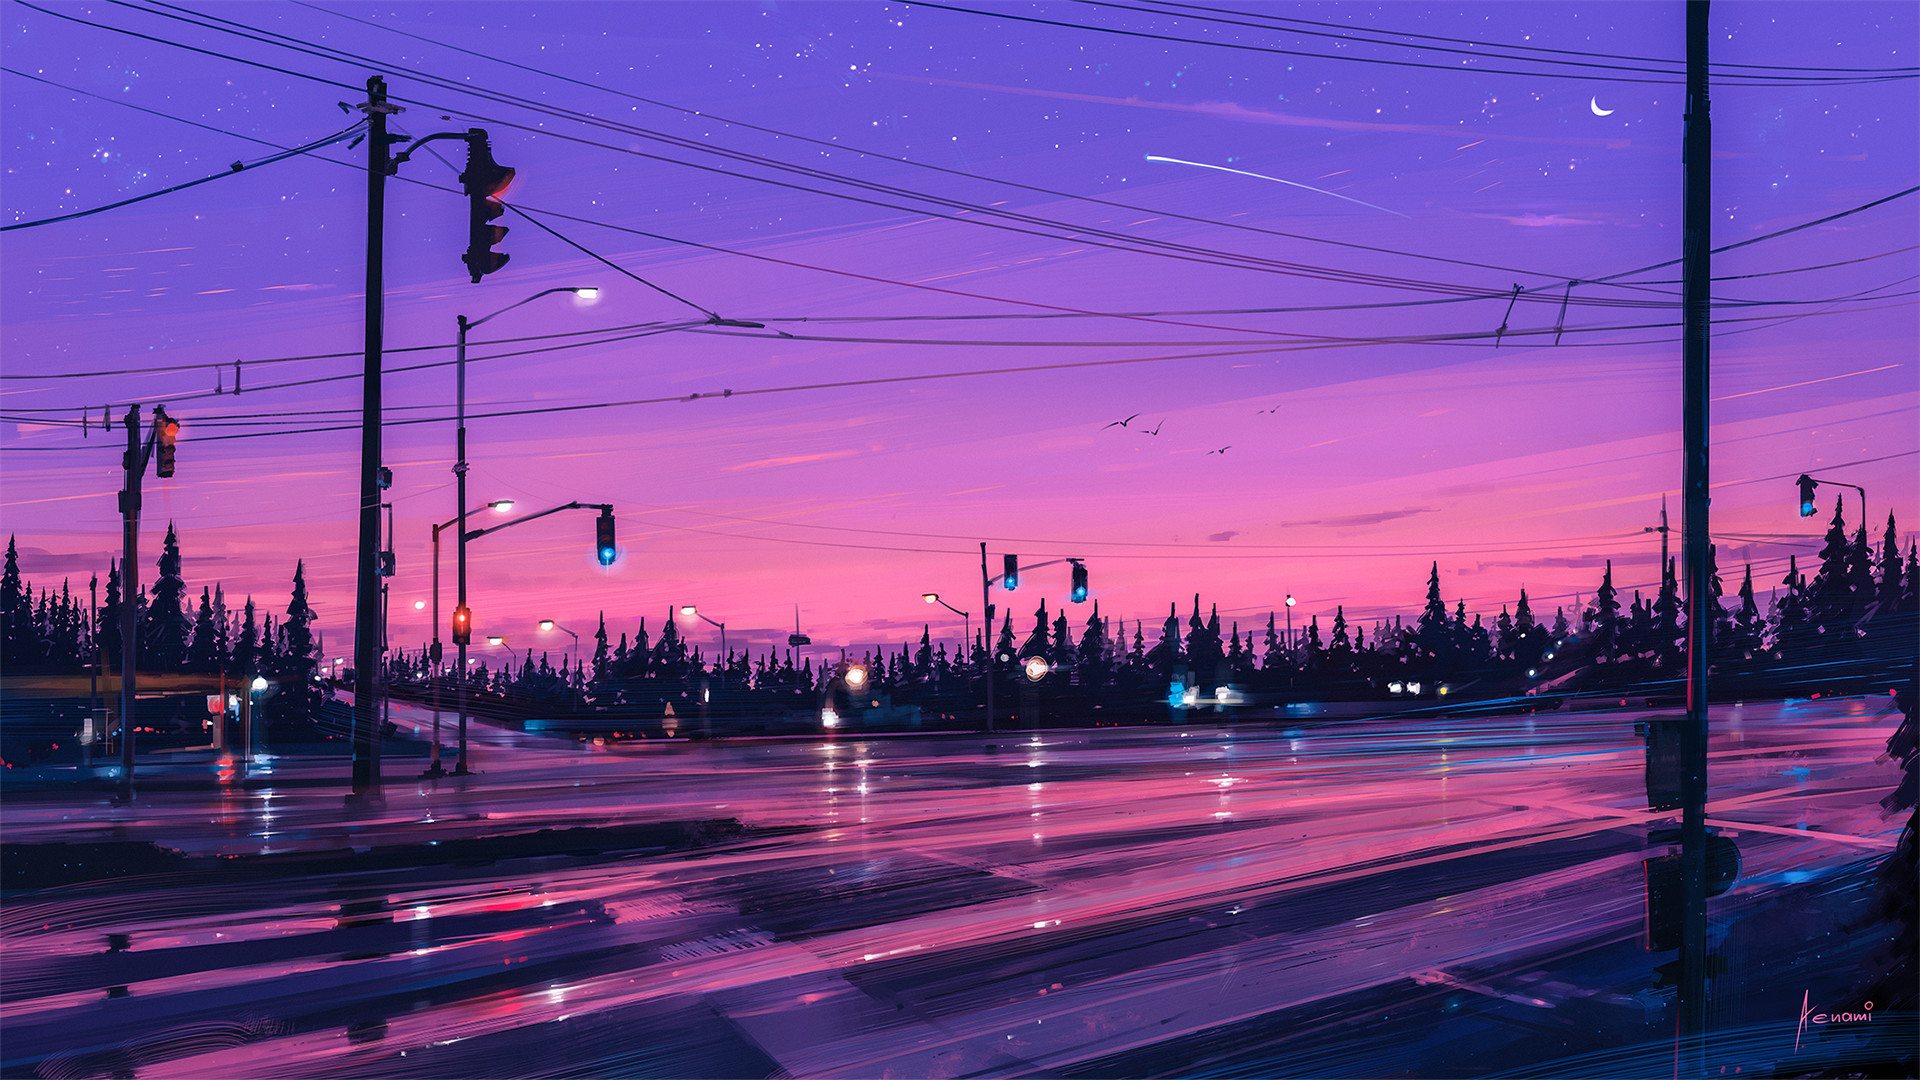
\includegraphics[width=0.75\textwidth]{alena-aenami-7p-m}
    \caption{Hello world}
    \label{fig:test-1}
\end{figure}

As you can see in figure \ref{fig:test-1} on page \pageref{fig:test-1}

\end{document}